\documentclass[svgnames,11pt]{beamer}
\input{/home/tof/Documents/Cozy/latex-include/preambule_commun.tex}
\input{/home/tof/Documents/Cozy/latex-include/preambule_beamer.tex}
%\usepackage{pgfpages} \setbeameroption{show notes on second screen=left}
\author[]{Christophe Viroulaud}
\title{Exercices Diviser pour régner}
\date{\framebox{\textbf{Algo 02}}}
%\logo{}
\institute{Terminale - NSI}

\begin{document}
\begin{frame}
    \titlepage
\end{frame}
\section{Exercice 1}
\begin{frame}[fragile]
    \frametitle{Exercice 1}

    \begin{center}
        \begin{lstlisting}[language=Python , basicstyle=\ttfamily\small, xleftmargin=2em, xrightmargin=2em]
def inserer(tab: list, j: int) -> None:
    if j >= 0 and tab[j] > tab[j+1]:
        tab[j], tab[j+1] = tab[j+1], tab[j]
        inserer(tab, j-1)


def tri_insertion_rec(tab: list) -> None:
    for i in range(len(tab)):
        inserer(tab, i-1)
\end{lstlisting}
    \end{center}

\end{frame}
\section{Exercice 2}
\begin{frame}[fragile]
    \frametitle{Exercice 2}
    La fonction \textbf{\texttt{inserer}} fait \emph{redescendre} l'élément de rang \emph{j} en le comparant avec celui de rang \emph{j-1}. Cette propagation \textbf{de proche en proche} s'arrête quand les deux éléments sont égaux. L'ordre relatif est préservé.
    \begin{center}
        \begin{lstlisting}[language=Python , basicstyle=\ttfamily\small, xleftmargin=2em, xrightmargin=2em]
t = [(1, 5), (3, 4), (1, 1), (2, 9), (1, 2)]
t = [(1, 5), (1, 1), (3, 4), (2, 9), (1, 2)]
t = [(1, 5), (1, 1), (2, 9), (3, 4), (1, 2)]
t = [(1, 5), (1, 1), (1, 2), (2, 9), (3, 4)]
\end{lstlisting}
        \captionof{code}{Exemple d'exécution du tri insertion}
        \label{CODE}
    \end{center}


\end{frame}
\begin{frame}
    \frametitle{}

    Dans le tri fusion, les éléments sont triés en se déplaçant également de proche en proche. L'ordre relatif est encore préservé.

\end{frame}
\begin{frame}[fragile]
    \frametitle{}

    \begin{center}
        \begin{lstlisting}[language=Python , basicstyle=\ttfamily\small, xleftmargin=1em, xrightmargin=1em]
def tri_selection(tab: list) -> None:
    for i in range(len(tab)):
        i_mini = i
        for j in range(i+1, len(tab)):
            if tab[j] < tab[i_mini]:
                i_mini = j
        tab[i], tab[i_mini] = tab[i_mini], tab[i]
\end{lstlisting}
        \captionof{code}{tri par sélection}
        \label{CODE}
    \end{center}

\end{frame}
\begin{frame}[fragile]
    \frametitle{}

    Dans un tableau de taille \emph{n}, le tri par sélection échange l'élément de rang \emph{j} par le plus petit dans l'intervalle $]j;n[$. Certains éléments peuvent ainsi \emph{sauter} par-dessus certains éléments égaux.
    \begin{center}
        \begin{lstlisting}[language=Python , basicstyle=\ttfamily\small, xleftmargin=1em, xrightmargin=1em]
t = [(1, 5), (2, 4), (1, 1), (2, 9), (1, 2)]
t = [(1, 5), (1, 1), (2, 4), (2, 9), (1, 2)]
t = [(1, 5), (1, 1), (1, 2), (2, 9), (2, 4)]
\end{lstlisting}
        \captionof{code}{Exemple de la non stabilité du tri par sélection}
        \label{CODE}
    \end{center}
\end{frame}
\section{Exercice 3}
\begin{frame}[fragile]
    \frametitle{Exercice 3}

    \begin{center}
        \begin{lstlisting}[language=Python , basicstyle=\ttfamily\small, xleftmargin=2em, xrightmargin=2em]
def dichotomie_imp(tab: int, x: int) -> int:
    debut, fin = 0, len(tab) - 1
    while debut <= fin:
        milieu = (debut + fin)//2
        if tab[milieu] == x:
            return milieu
        elif tab[milieu] < x:
            debut = milieu+1
        else:
            fin = milieu-1
    return -1
\end{lstlisting}
        \captionof{code}{Version impérative}
        \label{CODE}
    \end{center}

\end{frame}
\begin{frame}[fragile]

    \begin{center}
        \begin{lstlisting}[language=Python , basicstyle=\ttfamily\small, xleftmargin=2em, xrightmargin=2em]
def dichotomie_rec(tab: list, x: int, debut: int, fin: int) -> int:
    if debut <= fin:
        milieu = (debut + fin)//2
        if tab[milieu] == x:
            return milieu
        elif tab[milieu] < x:
            return dichotomie_rec(tab, x, milieu + 1, fin)
        else:
            return dichotomie_rec(tab, x, debut, milieu - 1)
    else:
        return -1
\end{lstlisting}
        \captionof{code}{Version récursive}
        \label{CODE}
    \end{center}

\end{frame}
\section{Exercice 4}
\begin{frame}
    \frametitle{Exercice 4}
\begin{center}
\centering
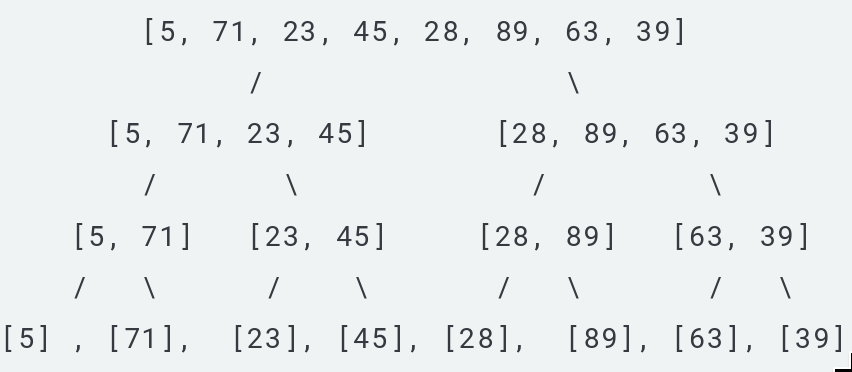
\includegraphics[width=8cm]{ressources/separation.png}
\captionof{figure}{Séparation}
\label{IMG}
\end{center}
\end{frame}
\begin{frame}
    \frametitle{}

    \begin{center}
        \centering
        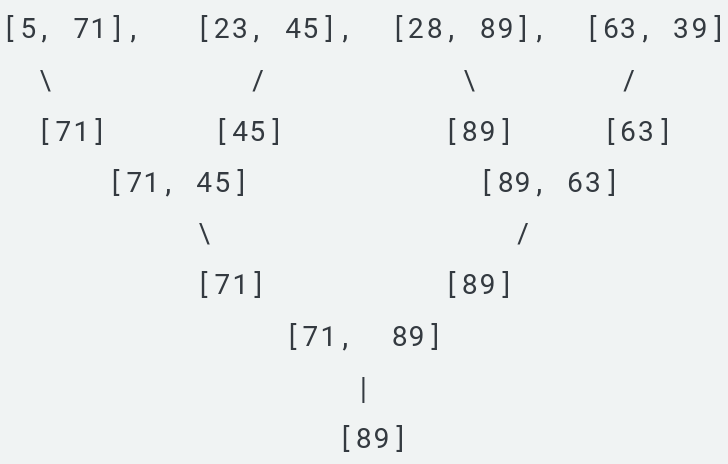
\includegraphics[width=8cm]{ressources/combinaison.png}
        \captionof{figure}{Recombinaison}
        \label{IMG}
        \end{center}
        Cette fonction renvoie le maximum de la liste.
\end{frame}
\begin{frame}
    \frametitle{}

    Complexité:
    \begin{itemize}
        \item À chaque appel récursif, la taille du tableau est divisé par 2. Comme pour le tri fusion, la complexité des appels est de l'ordre de $\log_2(n)$.
        \item À chaque remontée d'appel, on compare deux éléments. Le nombre de comparaisons dépend du niveau. Le total des comparaisons est de l'ordre de $n$.
    \end{itemize}
    \begin{center}
        \begin{tikzpicture}[scale=0.7, transform shape]
            \node[draw, minimum height=.7cm,minimum width = .7cm] (50) at (2.45,6) {16};
            \foreach \i in {0,1}
                {\node[draw, minimum height=.7cm,minimum width = .7cm] (4\i) at (1.05+2.8*\i,5) {8};}
            \foreach \i/\j in {00/0,01/1,10/2,11/3}
                {\node[draw, minimum height=.7cm,minimum width = .7cm] (3\i) at (.35+1.4*\j,4) {4};}
            \foreach \i/\j in {000/0,001/1,010/2,011/3,100/4,101/5,110/6,111/7}
                {\node[draw, minimum height=.7cm,minimum width = .7cm] (2\i) at (.7*\j,3) {2};}

            \foreach \i in {0,1}
                {\draw (50.south) -- (4\i.north);}
            \foreach \i in {0,1}{
                \foreach \j in {0,1}
                {\draw (4\i.south) -- (3\i\j.north);}
                }
            \foreach \i in {00,01,10,11}{
                \foreach \j in {0,1}
                {\draw (3\i.south) -- (2\i\j.north);}
                }
            
                \draw (8,7) node{comparaisons};
                \draw (8,6) node{$\dfrac{n}{16}$};
                \draw (8,5) node{$\dfrac{n}{8}$};
                \draw (8,4) node{$\dfrac{n}{4}$};
                \draw (8,3) node{$\dfrac{n}{2}$};
        \end{tikzpicture}
        \captionof{figure}{Exemple avec un tableau de 16 éléments}
    \end{center}
    La complexité est quasi-linéaire $n×\log(n)$.
\end{frame}
\section{Exercice 5}
\begin{frame}[fragile]
    \frametitle{Exercice 5}

\begin{center}
\begin{lstlisting}[language=Python , basicstyle=\ttfamily\small, xleftmargin=1em, xrightmargin=.5em]
def tri_rapide(tab: list) -> list:
    if not tab:
        return []
    else:
        pivot = tab[0]
        petit = [x for x in tab if x < pivot]
        grand = [x for x in tab[1:] if x >= pivot]
        return tri_rapide(petit) + [pivot] + tri_rapide(grand)
\end{lstlisting}
\end{center}  

\end{frame}
\begin{frame}[fragile]
    \frametitle{Exercice 5}

\begin{center}
\begin{lstlisting}[language=Python , basicstyle=\ttfamily\small, xleftmargin=1em, xrightmargin=1em]
def partitionner(tab: list, deb: int, fin: int) -> int:
    pivot = tab[deb]
    pos = deb
    for i in range(deb+1, fin):
        if tab[i] < pivot:
            pos += 1
            tab[i], tab[pos] = tab[pos], tab[i]
    # place le pivot
    tab[deb], tab[pos] = tab[pos], tab[deb]
    return pos
\end{lstlisting}
\end{center}  

\end{frame}
\begin{frame}[fragile]
    \frametitle{Exercice 5}

\begin{center}
\begin{lstlisting}[language=Python , basicstyle=\ttfamily\small, xleftmargin=1em, xrightmargin=1em]
def tri_rapide(tab: list, deb: int, fin: int) -> None:
    """
    Args:
        tab (list): tableau d'entiers
        deb (int): indice de début (inclus)
        fin (int): indice de fin (exclus)
    """
    if deb < fin:
        pivot = partitionner(tab, deb, fin)
        tri_rapide(tab, deb, pivot)
        tri_rapide(tab, pivot+1, fin)
\end{lstlisting}
\end{center}  

\end{frame}
\end{document}